\documentclass{article}

\usepackage[utf8x]{inputenc}
\usepackage[T1]{fontenc}
\usepackage[english]{babel}
\usepackage[left=2.5cm,top=2cm,right=2.5cm,bottom=2cm,nohead,foot=1cm]{geometry}
\usepackage[unicode]{hyperref}
\usepackage[absolute]{textpos}
\usepackage{setspace}
\usepackage{palatino}
\usepackage{lastpage}
\usepackage{fancyhdr}
\usepackage{graphicx}

\setlength{\TPHorizModule}{\paperwidth}\setlength{\TPVertModule}{\paperheight}

\def\name{Dr. Kliment Olechnovič}

\def\footerlink{}

\hypersetup{
  colorlinks = true,
  urlcolor = blue,
  pdfauthor = {\name},
  pdfkeywords = {curriculum vitae, bioinformatics, computer science, protein structure},
  pdftitle = {\name: Curriculum Vitae},
  pdfsubject = {Curriculum Vitae},
  pdfpagemode = UseNone
}

\setlength\parindent{0em}

\newenvironment{enumerate_tight}{
\begin{enumerate}
  \setlength{\itemsep}{4pt}
  \setlength{\parskip}{0pt}
  \setlength{\parsep}{0pt}
}{\end{enumerate}}

\newenvironment{itemize_tight}{
\begin{itemize}
  \setlength{\itemsep}{4pt}
  \setlength{\parskip}{0pt}
  \setlength{\parsep}{0pt}
}{\end{itemize}}

\renewcommand{\arraystretch}{1.4}

\pagestyle{fancy}
\fancyhf{}
\renewcommand{\headrulewidth}{0pt}
\renewcommand{\footrulewidth}{0pt}
\cfoot{Page \thepage\ of \pageref*{LastPage}}


\begin{document}

\begin{minipage}{0.80\linewidth}
\begin{center}
{\huge \bf \name}
\end{center}

\begin{center}
{\Large Curriculum Vitae}
\end{center}
\end{minipage}
\begin{minipage}{0.20\linewidth}
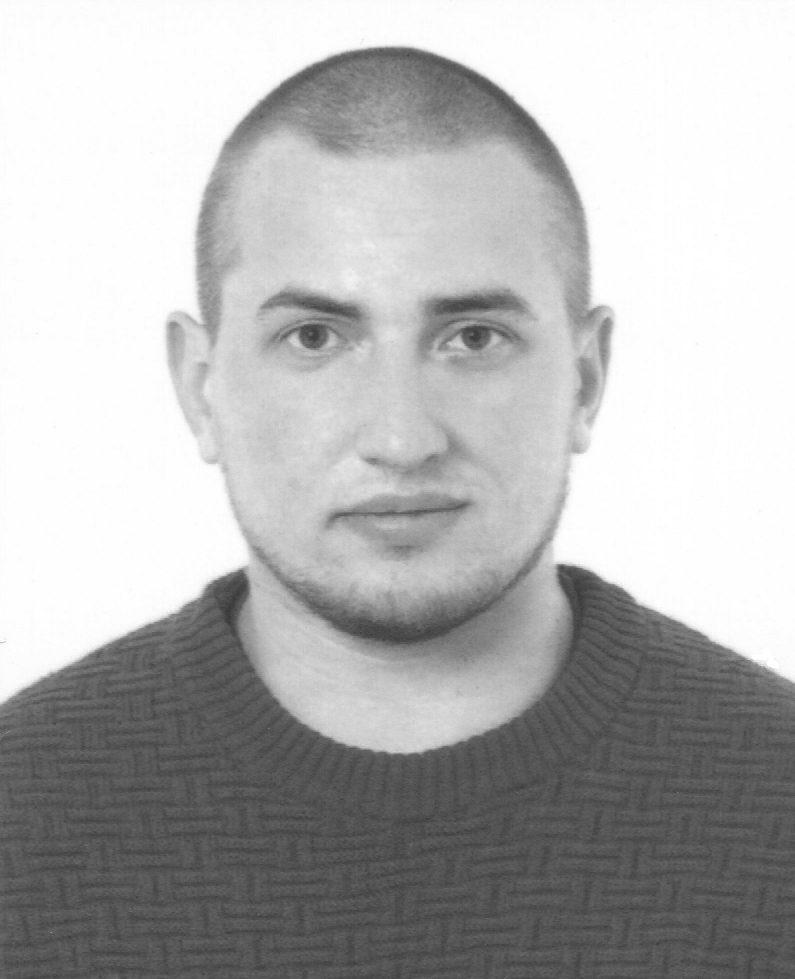
\includegraphics[width=\linewidth]{photo.jpg}
\end{minipage}


\section*{Main research interests}

\begin{minipage}{0.3\linewidth}
\begin{itemize_tight}
  \item Structural bioinformatics
  \item Machine learning
\end{itemize_tight}
\end{minipage}
\begin{minipage}{0.7\linewidth}
\begin{itemize_tight}
  \item Computational geometry
  \item Parallel computing
\end{itemize_tight}
\end{minipage}

\section*{Contact information}
\begin{tabular}{p{0.12\textwidth}p{0.85\textwidth}}
Email:               & \href{mailto:kliment.olechnovic@bti.vu.lt}{\tt kliment.olechnovic@bti.vu.lt} \\
Address:             & Saulėtekio 7, LT-10257 Vilnius \\
\end{tabular}


\section*{Online profiles}

\subsection*{Publications}
\begin{tabular}{p{0.20\textwidth}p{0.77\textwidth}}
Google Scholar:             & \href{https://scholar.google.lt/citations?user=uT_t5ewAAAAJ}{\tt https://scholar.google.lt/citations?user=uT\_t5ewAAAAJ} \\
ORCID:                      & \href{https://orcid.org/0000-0003-4918-9505}{\tt https://orcid.org/0000-0003-4918-9505} \\
PubMed:                     & \href{https://www.ncbi.nlm.nih.gov/pubmed/?term=Olechnovi%C4%8D+K%5BAuthor%5D}{\tt https://www.ncbi.nlm.nih.gov/pubmed/?term=Olechnovič+K[Author]} \\
\end{tabular}

\subsection*{Software}
\begin{tabular}{p{0.20\textwidth}p{0.77\textwidth}}
Bitbucket:       & \href{https://bitbucket.org/kliment}{\tt https://bitbucket.org/kliment} \\
\end{tabular}


\section*{Education}
\begin{tabular}{p{0.12\textwidth}p{0.05\textwidth}p{0.80\textwidth}}
2012 -- 2017 & Ph.D. & Computer Science, Vilnius University \\
2010 -- 2012 & M.S.  & Computer Science, Vilnius University (\emph{Magna Cum Laude}) \\
2005 -- 2009 & B.S.  & Bioinformatics, Vilnius University
\end{tabular}


\section*{Work experience}
\begin{tabular}{p{0.12\textwidth}p{0.85\textwidth}}
2017 -- now  & Research Scientist (Vilnius University / Life Sciences Center / Institute of Biotechnology)\\
2013 -- 2017 & Junior Research Scientist (Vilnius University / Institute of Biotechnology) \\
2010 -- 2013 & Research Engineer (Vilnius University / Institute of Biotechnology) \\
2009 -- 2010 & Research Engineer (Institute of Biotechnology, Vilnius) \\
2007 -- 2009 & C++ software developer (4Team Corporation, Vilnius)
\end{tabular}

\section*{Publications}

\subsection*{Papers in peer-reviewed journals}
\begin{enumerate_tight}
  \item Justas Dapkūnas, \underline{Kliment Olechnovič}, Česlovas Venclovas.
        \emph{Structural modeling of protein complexes: current capabilities and challenges}.
        Proteins (2019) doi:10.1002/prot.25774.
  \item Jianlin Cheng, Myong-Ho Choe, Arne Elofsson, Kun-Sop Han, Jie Hou, Ali H. A. Maghrabi, Liam J. McGuffin, David Menéndez-Hurtado, \underline{Kliment Olechnovič}, Torsten Schwede, Gabriel Studer, Karolis Uziela, Česlovas Venclovas, Björn Wallner.
        \emph{Estimation of model accuracy in CASP13}.
        Proteins (2019) doi:10.1002/prot.25767.
  \item \underline{Kliment Olechnovič}, Česlovas Venclovas.
        \emph{VoroMQA web server for assessing three-dimensional structures of proteins and protein complexes}.
        Nucleic Acids Res. (2019) doi:10.1093/nar/gkz367.
  \item \underline{Kliment Olechnovič}, Bohdan Monastyrskyy, Andriy Kryshtafovych, Česlovas Venclovas.
        \emph{Comparative analysis of methods for evaluation of protein models against native structures}.
        Bioinformatics (2019) 35 (6): 937-944.
  \item Justas Dapkūnas, \underline{Kliment Olechnovič}, Česlovas Venclovas.
        \emph{Modeling of protein complexes in CAPRI Round 37 using template-based approach combined with model selection}.
        Proteins (2018) 86 (Suppl 1): 292-301.
  \item \underline{Kliment Olechnovič}, Česlovas Venclovas.
        \emph{VoroMQA: Assessment of protein structure quality using interatomic contact areas}.
        Proteins (2017) 85 (6): 1131-1145. \emph{Featured on the cover}.
  \item Justas Dapkūnas, Albertas Timinskas, \underline{Kliment Olechnovič}, Mindaugas Margelevičius, Rytis Dičiūnas, Česlovas Venclovas.
        \emph{The PPI3D web server for searching, analyzing and modeling protein-protein interactions in the context of 3D structures}.
        Bioinformatics (2017) 33 (6): 935-937.
  \item \underline{Kliment Olechnovič}, Česlovas Venclovas.
        \emph{The CAD-score web server: contact area-based comparison of structures and interfaces of proteins, nucleic acids and their complexes}.
        Nucleic Acids Res. (2014) 42 (W1): 259-263. \emph{NAR Breakthrough Article}.
  \item \underline{Kliment Olechnovič}, Česlovas Venclovas.
        \emph{The use of interatomic contact areas to quantify discrepancies between RNA 3D models and reference structures}.
        Nucleic Acids Res. (2014) 42 (9): 5407-5415.
  \item \underline{Kliment Olechnovič}, Česlovas Venclovas.
        \emph{Voronota: A fast and reliable tool for computing the vertices of the Voronoi diagram of atomic balls}.
        J. Comput. Chem. (2014) 35 (8): 672-681.
  \item \underline{Kliment Olechnovič}, Eleonora Kulberkytė, Česlovas Venclovas.
        \emph{CAD-score: a new contact area difference-based function for evaluation of protein structural models}.
        Proteins (2013) 81 (1): 149-162.
  \item \underline{Kliment Olechnovič}, Mindaugas Margelevičius, Česlovas Venclovas.
        \emph{Voroprot: an interactive tool for the analysis and visualization of complex geometric features of protein structure}.
        Bioinformatics (2011) 27 (5): 723-724.
\end{enumerate_tight}

\subsection*{Book chapters}
\begin{itemize_tight}
  \item Visvaldas Kairys, \underline{Kliment Olechnovič}, Vytautas Raškevičius, Daumantas Matulis.
        \emph{In Silico Modeling of Inhibitor Binding to Carbonic Anhydrases}.
        Book chapter, Carbonic Anhydrase as Drug Target (2019), 215-232.
\end{itemize_tight}

\subsection*{Other publications}
\begin{itemize_tight}
  \item \underline{Kliment Olechnovič}.
        \emph{Methods for the analysis and assessment of the three-dimensional structures of proteins and nucleic acids: development and applications}.
        Doctoral dissertation, Vilnius University (2017).
  \item Justas Dapkūnas, \underline{Kliment Olechnovič}.
        \emph{Kompiuteriai padeda pažinti sudėtingą baltymų pasaulį}.
        Popular science article, SPECTRUM journal (2017), 1(26), ISSN 1822-0147.
\end{itemize_tight}

\subsection*{Presentations}
\begin{itemize_tight}
  \item 5 oral presentations at international conferences
  \item 15 poster presentations at international conferences (3 awards for best poster).
\end{itemize_tight}


\section*{Awards}
\begin{tabular}{p{0.12\textwidth}p{0.85\textwidth}}
2018 & Laureate of the ,,Best doctoral dissertation of 2017 in Lithuania'' contest \\
2015 & Lithuanian Academy of Sciences award for the best works by young researchers in 2014 \\
2013, 2014 & The Research Council of Lithuania scholarship for PhD students actively conducting scientific research \\
2013 & INFOBALT incentive scholarship for young scientists
\end{tabular}


\section*{Other achievements}
\begin{tabular}{p{0.12\textwidth}p{0.85\textwidth}}
2018 & Contributed to the best results in modeling structures of protein complexes
       in the world-wide CASP (Critical Assessment of Techniques for Protein Structure Prediction)
       and CAPRI (Critical Assessment of PRedicted Interactions) experiments \\
2018 & Top results in EMA (estimation of model accuracy)
       in the world-wide CASP experiment \\
2016 & Contributed to the best results in modeling structures of protein complexes
       in the world-wide CAPRI experiment \\
2016 & Top results in protein structure prediction
       in the world-wide CASP experiment
\end{tabular}


\section*{Languages}
\begin{tabular}{p{0.12\textwidth}p{0.85\textwidth}}
English        & full professional proficiency \\
Lithuanian     & native or bilingual proficiency \\
Russian        & native or bilingual proficiency
\end{tabular}

\end{document}
